\documentclass{presentatiesmetlogo}
\usepackage{graphicx}
\usepackage{color}
\usepackage{amsmath}
\usepackage{amsfonts}
\usepackage{amssymb}
\usepackage{verbatim}

\setlength{\unitlength}{1cm}
\newcommand{\ba}{\mbox{{\boldmath $a$}}}
\newcommand{\bA}{\mbox{{\boldmath $A$}}}
\newcommand{\bb}{\mbox{{\boldmath $b$}}}
\newcommand{\bB}{\mbox{{\boldmath $B$}}}
\newcommand{\bc}{\mbox{{\boldmath $c$}}}
\newcommand{\bC}{\mbox{{\boldmath $C$}}}
\newcommand{\bd}{\mbox{{\boldmath $d$}}}
\newcommand{\bD}{\mbox{{\boldmath $D$}}}
\newcommand{\be}{\mbox{{\boldmath $e$}}}
\newcommand{\bE}{\mbox{{\boldmath $E$}}}
\newcommand{\bbf}{\mbox{{\boldmath $f$}}}
\newcommand{\bF}{\mbox{{\boldmath $F$}}}
\newcommand{\bg}{\mbox{{\boldmath $g$}}}
\newcommand{\bG}{\mbox{{\boldmath $G$}}}
\newcommand{\bh}{\mbox{{\boldmath $h$}}}
\newcommand{\bH}{\mbox{{\boldmath $H$}}}
\newcommand{\bi}{\mbox{{\boldmath $i$}}}
\newcommand{\bI}{\mbox{{\boldmath $I$}}}
\newcommand{\bfI}{\mathbf{I}}
\newcommand{\bj}{\mbox{{\boldmath $j$}}}
\newcommand{\bJ}{\mbox{{\boldmath $J$}}}
\newcommand{\bk}{\mbox{{\boldmath $k$}}}
\newcommand{\bK}{\mbox{{\boldmath $K$}}}
\newcommand{\bl}{\mbox{{\boldmath $l$}}}
\newcommand{\bL}{\mbox{{\boldmath $L$}}}
\newcommand{\bm}{\mbox{{\boldmath $m$}}}
\newcommand{\bM}{\mbox{{\boldmath $M$}}}
\newcommand{\bn}{\mbox{{\boldmath $n$}}}
\newcommand{\bN}{\mbox{{\boldmath $N$}}}
\newcommand{\bo}{\mbox{{\boldmath $o$}}}
\newcommand{\bO}{\mbox{{\boldmath $O$}}}
\newcommand{\bp}{\mbox{{\boldmath $p$}}}
\newcommand{\bP}{\mbox{{\boldmath $P$}}}
\newcommand{\bq}{\mbox{{\boldmath $q$}}}
\newcommand{\bQ}{\mbox{{\boldmath $Q$}}}
\newcommand{\br}{\mbox{{\boldmath $r$}}}
\newcommand{\bR}{\mbox{{\boldmath $R$}}}
\newcommand{\bs}{\mbox{{\boldmath $s$}}}
\newcommand{\bS}{\mbox{{\boldmath $S$}}}
\newcommand{\bt}{\mbox{{\boldmath $t$}}}
\newcommand{\bT}{\mbox{{\boldmath $T$}}}
\newcommand{\bu}{\mbox{{\boldmath $u$}}}
\newcommand{\bU}{\mbox{{\boldmath $U$}}}
\newcommand{\bv}{\mbox{{\boldmath $v$}}}
\newcommand{\bV}{\mbox{{\boldmath $V$}}}
\newcommand{\bw}{\mbox{{\boldmath $w$}}}
\newcommand{\bW}{\mbox{{\boldmath $W$}}}
\newcommand{\bx}{\mbox{{\boldmath $x$}}}
\newcommand{\bX}{\mbox{{\boldmath $X$}}}
\newcommand{\by}{\mbox{{\boldmath $y$}}}
\newcommand{\bY}{\mbox{{\boldmath $Y$}}}
\newcommand{\bz}{\mbox{{\boldmath $z$}}}
\newcommand{\bZ}{\mbox{{\boldmath $Z$}}}

\newcommand{\bfalpha}{\mbox{{\boldmath $\alpha$}}}
\newcommand{\bfbeta}{\mbox{{\boldmath $\beta$}}}
\newcommand{\bfgamma}{\mbox{{\boldmath $\gamma$}}}
\newcommand{\bfdelta}{\mbox{{\boldmath $\delta$}}}
\newcommand{\eps}{\varepsilon}
\newcommand{\bfeps}{\mbox{{\boldmath $\varepsilon$}}}
\newcommand{\bfeta}{\mbox{{\boldmath $\eta$}}}
\newcommand{\bftheta}{\mbox{{\boldmath $\theta$}}}
\newcommand{\bfmu}{\mbox{{\boldmath $\mu$}}}
\newcommand{\bfpi}{\mbox{{\boldmath $\pi$}}}
\newcommand{\bfsigma}{\mbox{{\boldmath $\sigma$}}}
\newcommand{\bfomega}{\mbox{{\boldmath $\omega$}}}
\newcommand{\bfPi}{\mbox{{\boldmath $\Pi$}}}
\newcommand{\bfSigma}{\mbox{{\boldmath $\Sigma$}}}
\newcommand{\bfPhi}{\mbox{{\boldmath $\Phi$}}}


\newcommand{\logit}{\mbox{logit}}
\newcommand{\expit}{\mbox{expit}}

\newcommand{\code}[1]{\textcolor{blue}{\texttt{#1}}}
\newcommand{\red}[1]{\textcolor{red}{#1}}
\newcommand{\blue}[1]{\textcolor{blue}{#1}}
\newcommand{\redbf}[1]{\textcolor{red}{\textbf{#1}}}
\newcommand{\bluebf}[1]{\textcolor{blue}{\textbf{#1}}}
\newcommand{\magentabf}[1]{\textcolor{magenta}{\textbf{#1}}}
\newcommand{\argmax}{\operatornamewithlimits{argmax}}
\newcommand{\rightarrowP}{\operatornamewithlimits{\rightarrow}}
\newcommand{\etal}{{\it et al., }}
\newcommand{\Rnsp}{\textsf{R}}
\newcommand{\R}{{\textsf{R} }}



\let \nl = \newline

\renewcommand{\arraystretch}{2}
\renewcommand{\congresname}{ \mbox{Courses for the Quantitative Researcher 2017 -- Introduction to R} }
\addtolength{\oddsidemargin}{1cm}

\begin{document}

\pagestyle{myheadings}
\font
\fivrm = cmr5
\relax
\input prepicte
\input pictex
\input postpict
\sffamily
\raggedright
\LARGE

\title{Courses for the Quantitative Researcher\\Introduction to R}
\author{{\bfseries Elrozy Andrinopoulou}\\
Department of Biostatistics, Erasmus University Medical Center\\
$\mbox{ }$\\\texttt{e.andrinopoulou@erasmusmc.nl}}
\date{Courses for the Quantitative Researcher 2017}

\maketitle
%======================================================
%======================================================
%======================================================
\titel{What is this Course About}
\bitem
\item Statistics have flourished in the recent years mainly
due to the possibility of doing complex analysis using computers
\nl
\item The most valuable tool of a modern quantitative researcher
is his/her personal computer
\bitemt
\item Many statistical software exist to do simple and specialized
analysis
\nl
\eitem
\item Analysts must learn not only how to use the software
but also what is behind
\eitem
%======================================================
\titel{What is this Course About (cont'd)}
\bitem
\item Therefore, the aim of this course is twofold:
\nl
\item \underline{Aim I:} learn the software
\bitemt
\item learn how to use the statistical programming language \redbf{R}
\nl
\eitemt
\item \underline{Aim II:} understand how the software works
\bitemt
\item learn the basic mathematical tools for statistics, which you
will later need to understand more advanced courses such as
\textbf{Repeated Measurements (CE08), Bayesian Statistics (CE09), etc.}
\nl
\eitemt
\eitem
%======================================================
\titel{Agenda}
\bitem
\item {\huge \underline{\textbf{Part I-A:}} Intro to \R}
\begin{enumerate}
\item Introduction
\newline
\newline
\bitemt
\item How does \R look like ?
\item What is \R ?
\item Why \R ?
\item Where do I get \R ?
\item How does \R work ?
\item How to get help in \R ?
\eitemt
\end{enumerate}
\eitem
%======================================================
\titel{Agenda (cont'd)}
\bitem
\item {\huge \underline{\textbf{Part I-B:}} Intro to R}
\bitemt
\item Using \R
\item Starting with examples
\item Using \R Commands
\item Most Frequently Used R Objects
\item Data Manipulation
\item Data Exploration
\item Indexing
\item Functions
\item Loops and Control Flow
\item Importing Data
\eitemt
\eitem
%======================================================
\titel{Agenda (cont'd)}
\bitem
\item {\huge \underline{\textbf{Part I-B:}} Intro to R}
\newline
\newline
\bitemt
\item Graphs
\item Statistical Tests
\item Regression Models
\item Saving your Work
\item Review of Key Points
\eitemt
\eitem
%======================================================
\titel{Agenda (cont'd)}
\bitem
\item {\huge \underline{\textbf{Part I-C:}} Intro to R}
\newline
\newline
\bitemt
\item Markdown
\eitemt
\eitem
%======================================================
\titel{Agenda (cont'd)}
\bitem
\item {\huge \underline{\textbf{Part II:}} Concepts in Mathematics and Statistics}
\item[] by Joost van Rosmalen \ldots
\eitem
%======================================================
\titel{Schedule for Part I}
\bitem
\item March 20: 10h00 - 13h00
\item March 21: 10h00 - 13h00
\item March 22: 10h00 - 13h00
\item March 23: 10h00 - 13h00
\eitem
%======================================================
\titel{Schedule for Part II}
\bitem
\item March 20: 14h00 - 17h00
\item March 21: 14h00 - 16h00
\item March 22: 14h00 - 17h00
\item March 23: 14h00 - 17h00
\eitem
%======================================================
\titel{Exams}
\bitem
\item One for each part of the course
\nl
\item Date: March 24, 14h00 - 17h00
\nl
\item Format: Multiple Choice questions
\nl
\item Open-book
\eitem
%======================================================
\titel{Structure \& Material for Part I}
\bitem
\item Lectures: slides interchanged with live \R sessions
\nl
\item In-between the lectures $\Rightarrow$ \red{Practice Sessions}
\bitemt
\item you will be asked to perform small tasks
\item solutions of the practicals available beforehand
\nl
\eitemt
\item Material
\bitemt
\item slides
\item \R code with the output \& \R code in soft format
\item \redbf{more than what we are going to cover!}
\eitemt
\eitem
%======================================================
\titel{Structure \& Material for Part I (cont'd)}
\bitem
\item You are welcome to try along
\nl
\item You are welcome to interrupt and ask questions
\eitem
%======================================================
\titel{References}
\bitem
\item Intro with applications in statistics
\bitemt
\item Dalgaard, P. (2008) \emph{Introductory Statistics with R,
2nd Ed}. New York: Springer-Verlag. (moderate)
\item Venables, W. and Ripley, B. (2002) \emph{Modern Applied
Statistics with S}. New York: Springer-Verlag. (advanced)
\nl
\eitemt
\item Programming
\bitemt
\item Venables, W. and Ripley, B. (2000) \emph{S Programming}.
New York: Springer-Verlag.
\item Chambers, J. (2008) \emph{Software for Data Analysis
Programming with R}.  New York: Springer-Verlag.
\eitemt
\eitem
%======================================================
\titel{References (cont'd)}
\bitem
\item More books that use \R (or S) can be found at:
\code{http://www.r-project.org/doc/bib/R-books.html}, or\\
    \code{http://www.r-project.org/doc/bib/R-jabref.html}
\eitem
%======================================================
\titel{References (cont'd)}
\bitem
\item \R ships with a number of helpful manuals (illustrated later)
\nl
\item Other manuals and helpful material are available on-line
via CRAN:\\\code{http://cran.r-project.org/other-docs.html}
\bitemt
\item `Simple R' by John Verzani
(\code{http://cran.r-project.org/doc/contrib/Verzani-SimpleR.pdf})
\item `R reference card' by Tom Short
(\code{http://cran.r-project.org/doc/contrib/Short-refcard.pdf})
\eitemt
\eitem
%======================================================
%\begin{comment}
%\titel{PC Info}
%\bitem
%\item To start the PC
%\bitemt
%\item account: \blue{r}
%\item Password: \blue{ research2012}
%\item Domain: \blue{student}
%\nl
%\eitemt
%\item The files that we will use during the course
%are located at: \blue{U:\textbackslash}
%\eitem
%\end{comment}
%======================================================
%======================================================
%======================================================
%======================================================
\newpage
\mbox{ }
\vspace{5cm}
\begin{center}
{\Huge \textbf{Part I-A}}
\end{center}
%======================================================
\titel{1 Introduction}
\bitem
\item A little bit of history
\bitemt
\item it was initiated in 1992 by Ross Ihaka and Robert
Gentleman at University of Auckland, New Zealand
\item in 1997 the R Core Team was established with renowned
members of the statistical computing community
\item nowadays, the R Core Team has grown and consists of
about 20 members, experts in computing
\eitemt
\eitem
%======================================================
\titel{1 Introduction (cont'd)}
\bitem
\item How does \R look like ?
\eitem
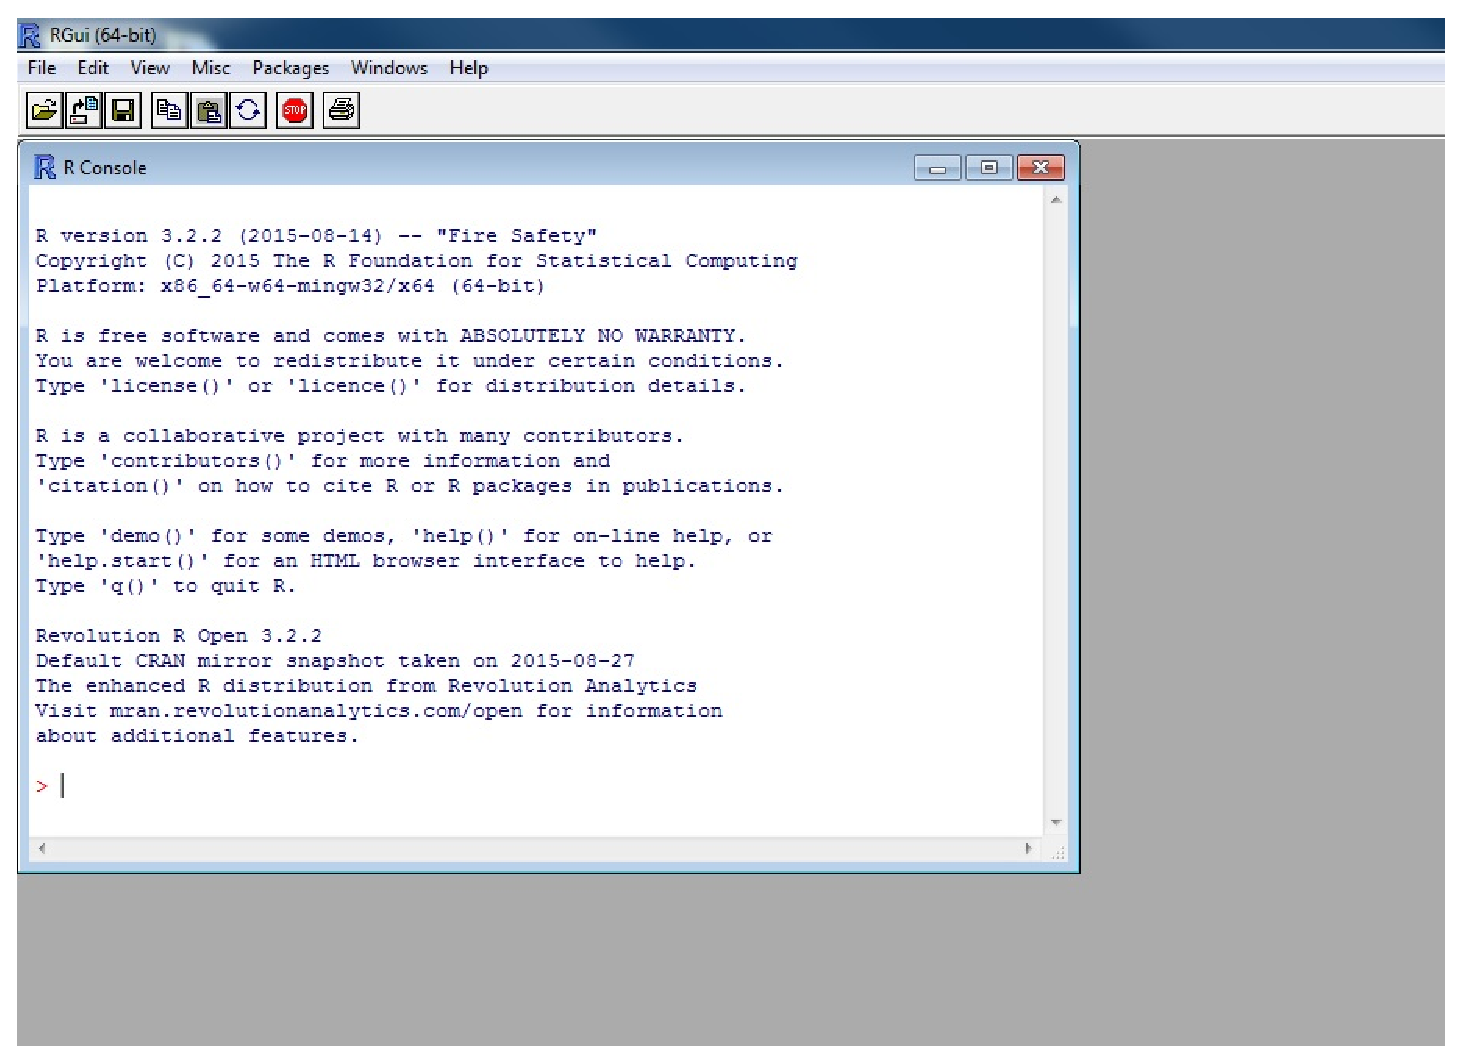
\includegraphics[scale=0.7]{Figures/R.eps}

%======================================================
\titel{1 Introduction (cont'd)}
\bitem
\item What is \R ?
\bitemt
\item is a software environment for statistical computing and graphics.
\item Unlike SPSS, \R is purely command driven
\eitemt
\eitem
%======================================================
\titel{1 Introduction (cont'd)}
\bitem
\item Why \R ?
\bitemt
\item R is a free software environment for statistical
computing and graphics.
\item it compiles and runs on LINUX, Windows and MacOS
\item R has extensive and powerful graphics \& data manipulation
capabilities
\item it can easily interface with low-level programming
languages, e.g., C/C++ or Fortran
\item it can be easily extended via R packages
\item the source code is available
\item users are allowed to modify and redistribute the code
\eitemt
\eitem
%======================================================
\titel{1 Introduction (cont'd)}
\bitem
\item Where do I get \R ?
\bitemt
\item \code{http://cran.r-project.org}
\item choose your platform, e.g., Windows, Linux
\item e.g., for Windows: \code{Windows} $\rightarrow$ \code{base}
$\rightarrow$ \code{Download R 3.3.3 for Windows}
\item Install $\ldots$
\nl
\eitemt
\eitem

%======================================================
\titel{1 Introduction (cont'd)}
\bitem
\item How does \R work ?
\bitemt
\item Packages built for specific tasks
\item Download \R packages from the CRAN web site $\Rightarrow$ within \R
\bitemt
\item[*] Packages
\item[*] Install package(s) $\ldots$
\item[*] make your choice(s)
\item[*] load the package using \code{library()} (\textcolor{red}{note}:
install does not mean load)
\eitemt
\eitemt
\eitem
%======================================================
\titel{1 Introduction (cont'd)}
\bitem
\item How does \R work ?
\eitem
\includegraphics[scale=0.5]{Figures/installpackages.eps}
%======================================================
\titel{1 Introduction (cont'd)}
\bitem
\item How does \R work ?
\eitem
\includegraphics[scale=0.5]{Figures/mean.eps}
%======================================================
\titel{1 Introduction (cont'd)}
\bitem
\item How to get help in \R ?
\bitemt
\item Within R
\bitemt
\item[*] \code{help.search("topic")} or \code{??"topic"} (depends on the
installed packages)
\item[*] \code{RSiteSearch("topic")} (requires internet connection)
\item[*] \code{help()} or \code{?} invoke the on-line help file for the
specified function
\item[*] checking the FAQ
\nl
\eitemt
\item On the internet
\bitemt
\item[*] \textsf{R}-help (\code{https://stat.ethz.ch/mailman/listinfo/r-help}
-- mailing list)
\item[*] \textsf{R}-seek (\code{http://www.rseek.org} -- Google-like
searched engine)
\item[*] \textsf{R}-wiki (\code{http://rwiki.sciviews.org/doku.php})
\eitemt
\eitemt
\eitem

%======================================================
\titel{1 Introduction (cont'd)}
\bitem
\item How to get help in \R ?
\bitemt
\item On the internet
\bitemt
\item[*] CRAN Task Views (\code{http://cran.r-project.org/web/views/}
-- categorization of packages)
\item[*] Crantastic (\code{http://crantastic.org/} -- categorization of
packages $+$ reviews)
\item[*] Equalis (\code{http://www.equalis.com/forums/} --
\textsf{R} forum)
\item[*] R4stats (\code{http://www.r4stats.com/} -- examples of basic \textsf{R} programs)
\item[*] R related Blogs (\code{http://www.r-bloggers.com/} -- many useful illustrations of \textsf{R} and \textsf{R} packages)
\eitemt
\eitemt
\eitem
%======================================================
\titel{1 Introduction (cont'd)}
\bitem
\item How to get help in \R ?
\eitem
\includegraphics[scale=0.5]{Figures/help.eps}
%======================================================
\titel{1 Introduction (cont'd)}
\bitem
\item How to get help in \R ?
\eitem
\includegraphics[scale=0.7]{Figures/help2.eps}
%======================================================
\titel{1 Introduction (cont'd)}
\bitem
\item Disadvantages of \R
\bitemt
\item appears intimidating to the first-time user
\item output is not so nice looking (but there are some alternatives)
\item exporting output is more difficult
\item cannot easily handle very very big data sets (depends on
the installed RAM)
\item a lot of things are available but it is sometimes hard to
find your way
\item the quality of the available packages is greatly varying
\eitemt
\eitem
%======================================================
%======================================================
%======================================================
%======================================================
\newpage
\mbox{ }
\vspace{5cm}
\begin{center}
{\Huge \textbf{Part I-B}}
\end{center}
%======================================================
\titel{1 Using \R}
\bitem
\item \R is a \textcolor{blue}{command}-based
\textcolor{red}{functional} language
\bitemt
\item write and execute \textcolor{blue}{commands}
\item use and define \textcolor{red}{functions}
\nl
\eitemt
\item You may write the commands in the R console (Windows)
or in a shell (Linux)
\nl
\nl
\nl
\nl
\fbox{\magentabf{You will become more familiar with the syntax as you use it}}
\eitem
%======================================================
\titel{1 Using \R (cont'd)}
\bitem
\item Strongly advisable to use a suitable text editor --
Some available options:
\bitemt
\item RWinEdt (for Windows; you also need WinEdt installed)
\item Tinn-R (for Windows; \code{http://sciviews.org/Tinn-R/})
\item Rkward (for Linux)
\item Rstudio (all major platforms; \code{http://www.rstudio.org/})
\item for more check
\code{http://www.sciviews.org/\_rgui/projects/Editors.html}
\eitemt
\eitem
%======================================================
\titel{1 Using \R (cont'd)}
\bitem
\item For this course: \textcolor{red}{Rstudio} (\code{http://www.rstudio.org/})
\bitemt
\item free
\item works fine in Windows, MacOS and Linux
\item helpful with errors
\eitemt
\eitem
%======================================================
\titel{1 Starting with Examples}
\begin{tabular}{cccc}
\textcolor{red}{patient} &  \textcolor{red}{height} &  \textcolor{red}{weight}  &  \textcolor{red}{sex} \\
 1& 1.608526& 65.80858&   male \\
 2& 1.800125& 63.45247&   male \\
 3& 1.694358& 66.75113& female \\
 4& 1.729665& 75.95356& female \\
 5& 1.420853& 71.79690&   male \\
 6& 1.671726& 59.96520&   male \\
 \vdots &&&
\end{tabular}
%======================================================
\titel{1 Starting with Examples (cont'd)}
\bitem
\item \fbox{What is a \textcolor{red}{matrix/vector}?}
\newline\newline
\item Common \textcolor{red}{questions}
\newline
\bitemt
\item What is the \textcolor{blue}{average} weight
\item What is the \textcolor{blue}{average} height
\item What is the \textcolor{blue}{average} height for \textcolor{blue}{males}?
\item What is the \textcolor{blue}{average} weight for \textcolor{blue}{females}?\
\item What is the \textcolor{blue}{average} BMI?
\item \dots
\eitemt
\eitem

%======================================================
\titel{1 Starting with Examples (cont'd)}
\begin{tabular}{cccc}
	\textcolor{red}{patient} &  \textbf{\textcolor{red}{height}} &  \textcolor{red}{weight}  &  \textcolor{red}{sex} \\
	1& \textbf{1.608526}& 65.80858&   male \\
	2& \textbf{1.800125}& 63.45247&   male \\
	3& \textbf{1.694358}& 66.75113& female \\
	4& \textbf{1.729665}& 75.95356& female \\
	5& \textbf{1.420853}& 71.79690&   male \\
	6& \textbf{1.671726}& 59.96520&   male \\
	\vdots &&&
\end{tabular}

%======================================================
\titel{1 Starting with Examples (cont'd)}
\bitem
\item What is a \textcolor{red}{matrix/vector}?
\newline\newline
\item Common \textcolor{red}{questions}
\newline
\bitemt
\item \fbox{What is the \textcolor{blue}{average} weight}
\item \fbox{What is the \textcolor{blue}{average} height}
\item What is the \textcolor{blue}{average} height for \textcolor{blue}{males}?
\item What is the \textcolor{blue}{average} weight for \textcolor{blue}{females}?\
\item What is the \textcolor{blue}{average} BMI?
\item \dots
\eitemt
\eitem
%======================================================
\titel{1 Using \R Commands (cont'd)}
\bitem
\item Elementary commands: \redbf{expressions} and
\bluebf{assignments}
\nl
\item An \redbf{expression} given as command is evaluated printed
and discarded
\nl
\item An \bluebf{assignment} evaluates an expression and passes the value to a
variable -- the result is not automatically printed
\eitem
%======================================================
\titel{1 Using \R Commands (cont'd)}
\bitem
\item Expression is given as a command,
\begin{verbatim}
> 10
[1] 10
\end{verbatim}
\item However, it cannot be viewed again unless the command is rerun.
\item In order to store information, the expression should assign the command
\begin{verbatim}
> x <- 10
> x
[1] 10
\end{verbatim}
\eitem
%======================================================
\titel{1 Using \R Commands (cont'd)}
\bitem
\item \R is case sensitive, e.g.,
\bitemt
\item \code{"sex"} is different than \code{"Sex"}
\nl
\eitemt
\item Commands are separated by a semi-colon or by a newline
\nl
\item Comments can be put anywhere, starting with a hashmark (\#): everything to the end of the line is a comment
\nl
\item Assign a value to an object by $<$- or =
\eitem
%======================================================
\titel{1 Using \R Commands (cont'd)}
\bitem
\item Missing values
\bitemt
\item are coded as \code{NA} (i.e., not available) \code{is.na()}
\nl
\eitemt
\item Infinity
\bitemt
\item is coded as \code{Inf} (plus infinity) or
\code{-Inf} (minus infinity) \code{is.finite()}
\nl
\eitemt
\eitem
%======================================================
\titel{2 Most Frequently Used \R Objects}
\bitem
\item Main types of \code{mode}s
\bitemt
\item \code{integer} \& \code{numeric}: quantitative data
\item \code{character}: qualitative data
\item \code{logical}: TRUE or FALSE
\item \code{list}: special \R object
\item \code{function}: see later
\nl
\eitemt
\item There are also other types of storage modes
(such as \code{raw}, \code{complex} and others)
but we are \textbf{not} going to use them in this course
-- for more info check \code{?mode}
\eitem
%======================================================
\titel{2 Most Frequently Used \R Objects (cont'd)}
\begin{tabular}{ccccc}
\textcolor{red}{patient} &  \textcolor{red}{height} &  \textcolor{red}{weight}  &  \textcolor{red}{sex} &  \textcolor{red}{weight 65higher} \\
 1& 1.608526& 65.80858&   male & TRUE\\
 2& 1.800125& 63.45247&   male & FALSE\\
 3& 1.694358& 66.75113& female & TRUE\\
 4& 1.729665& 75.95356& female & TRUE\\
 5& 1.420853& 71.79690&   male & TRUE\\
 6& 1.671726& 59.96520&   male & FALSE\\
 \vdots &&&&
\end{tabular}
%======================================================
\titel{2 Most Frequently Used \R Objects (cont'd)}
\bitem
\item In order to list the created objects use \code{objects()}
\begin{verbatim}
> objects()
# Now remove all objects
> rm(list=ls(all=TRUE))
> objects()
character(0)
\end{verbatim}
\item In order to investigate a specific object \redbf{dat} \code{str(dat)}
\eitem
%======================================================
\titel{2 Most Frequently Used \R Objects (cont'd)}
\bitem
\item Common \textcolor{red}{questions}
\newline
\bitemt
\item What is the \textcolor{blue}{average} weight?
\item What is the \textcolor{blue}{average} height?
\item What is the \textcolor{blue}{average} height for \textcolor{blue}{males}?
\item What is the \textcolor{blue}{average} weight for \textcolor{blue}{females}?\
\item \fbox{What is the \textcolor{blue}{average} BMI?}
\item \dots
\eitemt
\eitem
%======================================================
\titel{2 Most Frequently Used \R Objects (cont'd)}
\bitem
\item Basic arithmetics
\bitemt
\item \code{+}, \code{-}, \code{*}, \code{/}, \code{\^}
\newline
\newline
\eitemt
\item Complicated arithmetics
\bitemt
\item \code{\%*\%}, \code{t()}, \code{\%/\%}
\eitemt
\eitem
%======================================================
\titel{2 Most Frequently Used \R Objects (cont'd)}
\bitem
\item \R is able to distinguish between vectors, matrices, dataframes and lists
\begin{verbatim}
> #Creating a vector consisting of 1,2, and 3
> vector1 <- c(1,2,3)
> vector1
[1] 1 2 3
> vector1 <- 1:3
> vector1
[1] 1 2 3
\end{verbatim}
\begin{verbatim}
> #Creating a non-numeric vector
> non.num.vector <- c("A","B","C")
> non.num.vector
[1] "A" "B" "C"
\end{verbatim}
\eitem
%======================================================
\titel{2 Most Frequently Used \R Objects (cont'd)}
\bitem
\item \R is able to distinguish between vectors, matrices, lists and dataframes
\begin{verbatim}
> #Running basic arithmetic operations
> vector1 + vector1
[1] 2 4 6
\end{verbatim}
\eitem
%======================================================
\titel{2 Most Frequently Used \R Objects (cont'd)}
\bitem
\item \bluebf{Matrices} have the same type of elements
\item \bluebf{Data.frames} and \bluebf{lists} do not need to have the same type of elements
\item \bluebf{Lists} may have elements of different length
\begin{verbatim}
> #create a matrix
> vector2 <- 1:4
> matrix(vector2, 2, 2)
     [,1] [,2]
[1,]    1    3
[2,]    2    4
\end{verbatim}
\eitem
%======================================================
\titel{2 Most Frequently Used \R Objects (cont'd)}
\bitem
\item \bluebf{Matrices} have the same type of elements
\item \bluebf{Data.frames} and \bluebf{lists} do not need to have the same type of elements
\item \bluebf{Lists} may have elements of different length
\begin{verbatim}
> #create a matrix
> vector2 <- 1:4
> matrix(vector2, 2, 2, byrow = TRUE)
     [,1] [,2]
[1,]    1    2
[2,]    3    4
\end{verbatim}
\eitem
%======================================================
\titel{2 Most Frequently Used \R Objects (cont'd)}
\bitem
\item \bluebf{Matrices} have the same type of elements
\item \bluebf{Data.frames} and \bluebf{lists} do not need to have the same type of elements
\item \bluebf{Lists} may have elements of different length
\begin{verbatim}
> mylist = list(names = c("Jack","Mary"),
child.ages = c(4,7,9,10,11))
> mylist
$names
[1] "Jack" "Mary"
$child.ages
[1]  4  7  9 10 11
\end{verbatim}
\eitem


%======================================================
\titel{2 Most Frequently Used \R Objects (cont'd)}
Differences between \bluebf{Matrices}, \bluebf{Data.frames} and \bluebf{lists}
\nl
\nl
\nl
\bluebf{Matrix}
$\begin{cases}
\begin{tabular}{cc}
\textcolor{red}{height} &  \textcolor{red}{weight}  \\
 1.608526& 65.80858\\
 1.800125& 63.45247\\
 1.694358& 66.75113\\
 1.729665& 75.95356\\
 1.420853& 71.79690\\
 1.671726& 59.96520\\
\end{tabular}
\end{cases}$


%======================================================
\titel{2 Most Frequently Used \R Objects (cont'd)}
Differences between \bluebf{Matrices}, \bluebf{Data.frames} and \bluebf{lists}
\nl
\nl
\nl
\bluebf{Data frame}
$\begin{cases}
\begin{tabular}{ccccc}
\textcolor{red}{patient} &  \textcolor{red}{height} &  \textcolor{red}{weight}  &  \textcolor{red}{sex} &  \textcolor{red}{weight 65higher} \\
 1& 1.608526& 65.80858&   male & TRUE\\
 2& 1.800125& 63.45247&   male & FALSE\\
 3& 1.694358& 66.75113& female & TRUE\\
 4& 1.729665& 75.95356& female & TRUE\\
 5& 1.420853& 71.79690&   male & TRUE\\
 6& 1.671726& 59.96520&   male & FALSE\\
\end{tabular}
\end{cases}$
%======================================================
\titel{2 Most Frequently Used \R Objects (cont'd)}
Differences between \bluebf{Matrices}, \bluebf{Data.frames} and \bluebf{lists}
\nl
\nl
\nl
\bluebf{List}
$\begin{cases}
\begin{tabular}{cccc}
  \textcolor{red}{height} &  \textcolor{red}{weight}  &  \textcolor{red}{format}  &  \textcolor{red}{$\#$patients per gender} \\
1.608526& 65.80858 & short format &female 65\\
1.800125& 63.45247&   & male 47\\
1.694358& 66.75113&& \\
1.729665& 75.95356& &\\
1.420853& 71.79690& &  \\
1.671726& 59.96520& &   \\
\end{tabular}
\end{cases}$
%======================================================
\titel{3 Data Manipulation}
\bitem
\item \code{numeric} variables to \code{factor}s
\nl
\item Compute new variables
\bitemt
\item transform variables
\nl
\eitemt
\item Matrices of \red{wide} $\Leftrightarrow$ \blue{long} format
\nl
\item Missing values and outliers
\eitem
%======================================================
\titel{3 Data Manipulation}
\begin{tabular}{cccccc}
\textcolor{red}{patient} &  \textcolor{red}{height} &   \textcolor{red}{sex} &  \textcolor{red}{weightBase} & \textcolor{red}{weight6m}  & \textcolor{red}{weight1y}\\
  \bluebf{1} &  \bluebf{1.61}  & \bluebf{male}    &  \bluebf{65.81}   & \bluebf{62.15}  &  \bluebf{60.47}\\
  2 &  1.80  & male   &   63.45  &  67.45  &  64.84\\
 3  & 1.69 &female    &  66.75   & 66.52  &  65.22\\
 4  & 1.73& female    &  75.95  &  77.14  &  79.52\\
   5 &  1.42 &  male  &    71.80  &  60.63 &   61.35\\
  6 &  1.67 &  male  &    59.97  &  58.84 &   54.83\\
 \vdots &&&&
\end{tabular}
%======================================================
\titel{3 Data Manipulation (cont'd)}
\begin{tabular}{ccccc}
\textcolor{red}{patient} &  \textcolor{red}{height} &   \textcolor{red}{sex} &  \textcolor{red}{time} & \textcolor{red}{weight}  \\
   \bluebf{1}  & \bluebf{1.61} & \bluebf{male} & \bluebf{baseline} &  \bluebf{65.81}\\
   \bluebf{1}  & \bluebf{1.61} & \bluebf{male} & \bluebf{6months} & \bluebf{62.15}\\
 \bluebf{1} &  \bluebf{1.61} & \bluebf{male}  &  \bluebf{1year} & \bluebf{60.47}\\
   2  & 1.80 &male& baseline & 63.45\\
    2 &  1.80 &male&  6months&  67.45\\
  2  & 1.80 &male  &  1year & 64.84\\
 \vdots &&&&
\end{tabular}
%======================================================
\titel{4 Data Exploration}
\bitem
\item Common \textcolor{red}{questions}
\newline
\bitemt
\item \fbox{What is the \textcolor{blue}{mean} and \textcolor{blue}{sd} for weight?}
\item What is the  \textcolor{blue}{mean} and \textcolor{blue}{sd} for height?
\item What is the \textcolor{blue}{mean} and \textcolor{blue}{sd} for weight in \textcolor{blue}{males}?
\item What is the \textcolor{blue}{mean} and \textcolor{blue}{sd} for height in \textcolor{blue}{females}?
\item What is the \textcolor{blue}{median} and \textcolor{blue}{interquartile range} for weight?
\item What is the \textcolor{blue}{mean} and \textcolor{blue}{sd} for BMI?
\item What is the  \textcolor{blue}{percentage} of males and females?
\eitemt
\eitem
%======================================================
\titel{4 Data Exploration  (cont'd)}
\bitem
\item Common \textcolor{red}{questions}
\newline
\bitemt
\item What is the \textcolor{blue}{mean} and \textcolor{blue}{sd} for weight?
\item \fbox{What is the \textcolor{blue}{mean} and \textcolor{blue}{sd} for height?}
\item What is the \textcolor{blue}{mean} and \textcolor{blue}{sd} for weight in \textcolor{blue}{males}?
\item What is the \textcolor{blue}{mean} and \textcolor{blue}{sd} for height in \textcolor{blue}{females}?
\item What is the \textcolor{blue}{median} and \textcolor{blue}{interquartile range} for weight?
\item What is the \textcolor{blue}{mean} and \textcolor{blue}{sd} for BMI?
\item What is the  \textcolor{blue}{percentage} of males and females?
\eitemt
\eitem
%======================================================
\titel{4 Data Exploration  (cont'd)}
\bitem
\item Common \textcolor{red}{questions}
\newline
\bitemt
\item What is the \textcolor{blue}{mean} and \textcolor{blue}{sd} for weight?
\item What is the \textcolor{blue}{mean} and \textcolor{blue}{sd} for height?
\item \fbox{What is the \textcolor{blue}{mean} and \textcolor{blue}{sd} for weight in \textcolor{blue}{males}?}
\item What is the \textcolor{blue}{mean} and \textcolor{blue}{sd} for height in \textcolor{blue}{females}?
\item What is the \textcolor{blue}{median} and \textcolor{blue}{interquartile range} for weight?
\item What is the \textcolor{blue}{mean} and \textcolor{blue}{sd} for BMI?
\item What is the  \textcolor{blue}{percentage} of males and females?
\eitemt
\eitem
%======================================================
\titel{4 Data Exploration  (cont'd)}
\bitem
\item Common \textcolor{red}{questions}
\newline
\bitemt
\item What is the \textcolor{blue}{mean} and \textcolor{blue}{sd} for weight?
\item What is the  \textcolor{blue}{mean} and \textcolor{blue}{sd} for height?
\item What is the \textcolor{blue}{mean} and \textcolor{blue}{sd} for weight in \textcolor{blue}{males}?
\item \fbox{What is the \textcolor{blue}{mean} and \textcolor{blue}{sd} for height in \textcolor{blue}{females}?}
\item What is the \textcolor{blue}{median} and \textcolor{blue}{interquartile range} for weight?
\item What is the \textcolor{blue}{mean} and \textcolor{blue}{sd} for BMI?
\item What is the  \textcolor{blue}{percentage} of males and females?
\eitemt
\eitem
%======================================================
\titel{4 Data Exploration  (cont'd)}
\bitem
\item Common \textcolor{red}{questions}
\newline
\bitemt
\item What is the \textcolor{blue}{mean} and \textcolor{blue}{sd} for weight?
\item What is the  \textcolor{blue}{mean} and \textcolor{blue}{sd} for height?
\item What is the \textcolor{blue}{mean} and \textcolor{blue}{sd} for weight in \textcolor{blue}{males}?
\item What is the \textcolor{blue}{mean} and \textcolor{blue}{sd} for height in \textcolor{blue}{females}?
\item \fbox{What is the \textcolor{blue}{median} and \textcolor{blue}{interquartile range} for weight?}
\item What is the \textcolor{blue}{mean} and \textcolor{blue}{sd} for BMI?
\item What is the  \textcolor{blue}{percentage} of males and females?
\eitemt
\eitem
%======================================================
\titel{4 Data Exploration  (cont'd)}
\bitem
\item Common \textcolor{red}{questions}
\newline
\bitemt
\item What is the \textcolor{blue}{mean} and \textcolor{blue}{sd} for weight?
\item What is the  \textcolor{blue}{mean} and \textcolor{blue}{sd} for height?
\item What is the \textcolor{blue}{mean} and \textcolor{blue}{sd} for weight in \textcolor{blue}{males}?
\item What is the \textcolor{blue}{mean} and \textcolor{blue}{sd} for height in \textcolor{blue}{females}?
\item What is the \textcolor{blue}{median} and \textcolor{blue}{interquartile range} for weight?
\item \fbox{What is the \textcolor{blue}{mean} and \textcolor{blue}{sd} for BMI?}
\item What is the  \textcolor{blue}{percentage} of males and females?
\eitemt
\eitem
%======================================================
\titel{4 Data Exploration  (cont'd)}
\bitem
\item Common \textcolor{red}{questions}
\newline
\bitemt
\item What is the \textcolor{blue}{mean} and \textcolor{blue}{sd} for weight?
\item What is the  \textcolor{blue}{mean} and \textcolor{blue}{sd} for height?
\item What is the \textcolor{blue}{mean} and \textcolor{blue}{sd} for weight in \textcolor{blue}{males}?
\item What is the \textcolor{blue}{mean} and \textcolor{blue}{sd} for height in \textcolor{blue}{females}?
\item What is the \textcolor{blue}{median} and \textcolor{blue}{interquartile range} for weight?
\item What is the \textcolor{blue}{mean} and \textcolor{blue}{sd} for BMI?
\item \fbox{What is the \textcolor{blue}{percentage} of males and females?}
\eitemt
\eitem
%======================================================
\titel{4 Data Exploration  (cont'd)}
\bitem
\item Common \textcolor{red}{questions} - for long format dataset
\newline
\bitemt
\item \fbox{What is the \textcolor{blue}{mean} weight per \textcolor{blue}{patient}?}
\item What is the \textcolor{blue}{mean} weight of all patients after \textcolor{blue}{1 year}?
\item What is the \textcolor{blue}{mean} weight of all patients at \textcolor{blue}{baseline}?
\eitemt
\eitem
%======================================================
\titel{4 Data Exploration  (cont'd)}
\bitem
\item Common \textcolor{red}{questions} - for long format dataset
\newline
\bitemt
\item What is the \textcolor{blue}{mean} weight per \textcolor{blue}{patient}?
\item \fbox{What is the \textcolor{blue}{mean} weight of all patients after \textcolor{blue}{1 year}?}
\item What is the \textcolor{blue}{mean} weight of all patients at \textcolor{blue}{baseline}?
\eitemt
\eitem
%======================================================
\titel{4 Data Exploration  (cont'd)}
\bitem
\item Common \textcolor{red}{questions} - for long format dataset
\newline
\bitemt
\item What is the \textcolor{blue}{mean} weight per \textcolor{blue}{patient}?
\item What is the \textcolor{blue}{mean} weight of all patients after \textcolor{blue}{1 year}?
\item \fbox{What is the \textcolor{blue}{mean} weight of all patients at \textcolor{blue}{baseline}?}
\eitemt
\eitem
%======================================================
%\titel{2 Most Frequently Used \R Objects (cont'd)}
%\bitem
%\item Every object in \R has a \code{class}
%\nl
%\item This dictates how (some) generic methods (e.g., \code{print},
%\code{summary}, etc.) deal with this object
%\nl
%\item Some common \R \code{class}es
%\bitemt
%\item \code{integer} \& \code{numeric}
%\item \code{character} \& \code{factor}
%\item \code{matrix}
%\item \code{list} \& \code{data.frame}
%\eitemt
%\eitem
%%======================================================
%\titel{2 Most Frequently Used \R Objects (cont'd)}
%\bitem
%\item The \code{str()} function
%\nl
%\item Sequences \& replicates
%\bitemt
%\item \code{seq()} and \code{":"}
%\item \code{rep()}
%\nl
%\eitemt
%\item Basic arithmetics
%\bitemt
%\item \code{+}, \code{-}, \code{*}, \code{/}, \code{\%/\%},
%\code{\%\%}, \code{\^}
%\item \code{\%*\%}, \code{t()}
%\eitemt
%\eitem
%======================================================
\titel{5 Indexing}
\bitem
\item Very powerful for data manipulation
\nl
\item Three basic types
\bitemt
\item position indexing
\item name indexing
\item logical indexing
\eitemt
\eitem
%======================================================
\titel{5 Indexing (cont'd)}
\bitem
\item Indexing for vectors and matrices
\nl
\item Special indexing for \code{list}s and \code{data.frame}s
\bitemt
\item the difference between \code{[}, \code{[[} and \code{\$}
\item indexing by row names (in \code{data.frame}s)
\nl
\eitemt
%\item Useful functions for indexing
%\bitemt
%\item \code{match()}, \code{\%in\%}
%\item \code{rep()}, \code{seq()}
%\item \code{which()}, \code{which.min()}, \code{which.max()}
%\item \code{cut()}, \code{duplicated()}
%\eitemt
\eitem
%======================================================
\titel{5 Indexing (cont'd)}
\bitem
\item \textcolor{red}{Position indexing}
\bitemt
\item \fbox{What is the 3rd element for vector height?}
\item What is the gender of the 10th patient?
\item What are the details of the 5th patient?
\nl
\eitemt
\item \textcolor{red}{Name indexing}
\bitemt
\item Print the vector sex
\eitemt
\eitem
%======================================================
\titel{5 Indexing (cont'd)}
\bitem
\item \textcolor{red}{Position indexing}
\bitemt
\item What is the 3rd element for vector height?
\item \fbox{What is the gender of the 10th patient?}
\item What are the details of the 5th patient?
\nl
\eitemt
\item \textcolor{red}{Name indexing}
\bitemt
\item Print the vector sex
\eitemt
\eitem
%======================================================
\titel{5 Indexing (cont'd)}
\bitem
\item \textcolor{red}{Position indexing}
\bitemt
\item What is the 3rd element for vector height?
\item What is the gender of the 10th patient?
\item \fbox{What are the details of the 5th patient?}
\nl
\eitemt
\item \textcolor{red}{Name indexing}
\bitemt
\item Print the vector sex
\eitemt
\eitem
%======================================================
\titel{5 Indexing (cont'd)}
\bitem
\item \textcolor{red}{Position indexing}
\bitemt
\item What is the 3rd element for vector height?
\item What is the gender of the 10th patient?
\item What are the details of the 5th patient?
\nl
\eitemt
\item \textcolor{red}{Name indexing}
\bitemt
\item \fbox{Print the vector sex}
\eitemt
\eitem
%======================================================
\titel{5 Indexing (cont'd)}
\bitem
\item \textcolor{red}{Logical expressions for indexing}
\bitemt
\item \fbox{What are the \textcolor{blue}{weights} for all \textcolor{blue}{females}?}
\item What are the \textcolor{blue}{heights} for all \textcolor{blue}{males}?
\item Print only the details for \textcolor{blue}{females}
\item What are the \textcolor{blue}{weights} for patients that are taller than \textcolor{blue}{1.65}?
\item What are the \textcolor{blue}{weights} for \textcolor{blue}{female} patients that are taller than \textcolor{blue}{1.70}?
\item What are the \textcolor{blue}{weights} for \textcolor{blue}{male} patients or patients taller than \textcolor{blue}{1.80}?
\item Select patients that have \textcolor{blue}{no missing values} in \textcolor{blue}{weight}
\item Keep the first measurement per \textcolor{blue}{patient}
\eitemt
\eitem
%======================================================
\titel{5 Indexing (cont'd)}
\bitem
\item \textcolor{red}{Logical expressions for indexing}
\bitemt
\item What are the \textcolor{blue}{weights} for all \textcolor{blue}{females}?
\item \fbox{What are the \textcolor{blue}{heights} for all \textcolor{blue}{males}?}
\item Print only the details for \textcolor{blue}{females}
\item What are the \textcolor{blue}{weights} for patients that are taller than \textcolor{blue}{1.65}
\item What are the \textcolor{blue}{weights} for \textcolor{blue}{female} patients that are taller than \textcolor{blue}{1.70}
\item What are the \textcolor{blue}{weights} for \textcolor{blue}{male} patients or patients taller than \textcolor{blue}{1.80}
\item Select patients that have \textcolor{blue}{no missing values} in \textcolor{blue}{weight}
\item Keep the first measurement per \textcolor{blue}{patient}
\eitemt
\eitem
%======================================================
\titel{5 Indexing (cont'd)}
\bitem
\item \textcolor{red}{Logical expressions for indexing}
\bitemt
\item What are the \textcolor{blue}{weights} for all \textcolor{blue}{females}?
\item What are the \textcolor{blue}{heights} for all \textcolor{blue}{males}?
\item \fbox{Print only the details for \textcolor{blue}{females}}
\item What are the \textcolor{blue}{weights} for patients that are taller than \textcolor{blue}{1.65}
\item What are the \textcolor{blue}{weights} for \textcolor{blue}{female} patients that are taller than \textcolor{blue}{1.70}
\item What are the \textcolor{blue}{weights} for \textcolor{blue}{male} patients or patients taller than \textcolor{blue}{1.80}
\item Select patients that have \textcolor{blue}{no missing values} in \textcolor{blue}{weight}
\item Keep the first measurement per \textcolor{blue}{patient}
\eitemt
\eitem
%======================================================
\titel{5 Indexing (cont'd)}
\bitem
\item \textcolor{red}{Logical expressions for indexing}
\bitemt
\item What are the \textcolor{blue}{weights} for all \textcolor{blue}{females}?
\item What are the \textcolor{blue}{heights} for all \textcolor{blue}{males}?
\item Print only the details for \textcolor{blue}{females}
\item \fbox{What are the \textcolor{blue}{weights} for patients that are taller than \textcolor{blue}{1.65}}
\item What are the \textcolor{blue}{weights} for \textcolor{blue}{female} patients that are taller than \textcolor{blue}{1.70}
\item What are the \textcolor{blue}{weights} for \textcolor{blue}{male} patients or patients taller than \textcolor{blue}{1.80}
\item Select patients that have \textcolor{blue}{no missing values} in \textcolor{blue}{weight}
\item Keep the first measurement per \textcolor{blue}{patient}
\eitemt
\eitem
%======================================================
\titel{5 Indexing (cont'd)}
\bitem
\item \textcolor{red}{Logical expressions for indexing}
\bitemt
\item What are the \textcolor{blue}{weights} for all \textcolor{blue}{females}?
\item What are the \textcolor{blue}{heights} for all \textcolor{blue}{males}?
\item Print only the details for \textcolor{blue}{females}
\item What are the \textcolor{blue}{weights} for patients that are taller than \textcolor{blue}{1.65}
\item \fbox{What are the \textcolor{blue}{weights} for \textcolor{blue}{female} patients that are taller than \textcolor{blue}{1.70}}
\item What are the \textcolor{blue}{weights} for \textcolor{blue}{male} patients or patients taller than \textcolor{blue}{1.80}
\item Select patients that have \textcolor{blue}{no missing values} in \textcolor{blue}{weight}
\item Keep the first measurement per \textcolor{blue}{patient}
\eitemt
\eitem
%======================================================
\titel{5 Indexing (cont'd)}
\bitem
\item \textcolor{red}{Logical expressions for indexing}
\bitemt
\item What are the \textcolor{blue}{weights} for all \textcolor{blue}{females}?
\item What are the \textcolor{blue}{heights} for all \textcolor{blue}{males}?
\item Print only the details for \textcolor{blue}{females}
\item What are the \textcolor{blue}{weights} for patients that are taller than \textcolor{blue}{1.65}
\item What are the \textcolor{blue}{weights} for \textcolor{blue}{female} patients that are taller than \textcolor{blue}{1.70}
\item \fbox{What are the \textcolor{blue}{weights} for \textcolor{blue}{male} patients or patients taller than \textcolor{blue}{1.80}}
\item Select patients that have \textcolor{blue}{no missing values} in \textcolor{blue}{weight}
\item Keep the first measurement per \textcolor{blue}{patient}
\eitemt
\eitem
%======================================================
\titel{5 Indexing (cont'd)}
\bitem
\item \textcolor{red}{Logical expressions for indexing}
\bitemt
\item What are the \textcolor{blue}{weights} for all \textcolor{blue}{females}?
\item What are the \textcolor{blue}{heights} for all \textcolor{blue}{males}?
\item Print only the details for \textcolor{blue}{females}
\item What are the \textcolor{blue}{weights} for patients that are taller than \textcolor{blue}{1.65}
\item What are the \textcolor{blue}{weights} for \textcolor{blue}{female} patients that are taller than \textcolor{blue}{1.70}
\item What are the \textcolor{blue}{weights} for \textcolor{blue}{male} patients or patients taller than \textcolor{blue}{1.80}
\item \fbox{Select patients that have \textcolor{blue}{no missing values} in \textcolor{blue}{weight}}
\item Keep the first measurement per \textcolor{blue}{patient}
\eitemt
\eitem
%======================================================
\titel{5 Indexing (cont'd)}
\bitem
\item \textcolor{red}{Logical expressions for indexing}
\bitemt
\item What are the \textcolor{blue}{weights} for all \textcolor{blue}{females}?
\item What are the \textcolor{blue}{heights} for all \textcolor{blue}{males}?
\item Print only the details for \textcolor{blue}{females}
\item What are the \textcolor{blue}{weights} for patients that are taller than \textcolor{blue}{1.65}
\item What are the \textcolor{blue}{weights} for \textcolor{blue}{female} patients that are taller than \textcolor{blue}{1.70}
\item What are the \textcolor{blue}{weights} for \textcolor{blue}{male} patients or patients taller than \textcolor{blue}{1.80}
\item Select patients that have \textcolor{blue}{no missing values} in \textcolor{blue}{weight}
\item \fbox{Keep the first measurement per \textcolor{blue}{patient}}
\eitemt
\eitem
%======================================================
\titel{6 Functions}
\bitem
\item What are functions \& how to define them
\bitemt
\item each package has several functions
\item functions $\Rightarrow$ a group of (organized) \R commands
\nl
\eitemt
\item Why to define functions
\bitemt
\item \R is a functional language
\item organize your code: easier to reuse and distribute to others
\item formal definition of arguments
\item it protects from dangerous use of variable names
\nl
\eitemt
%\item Lexical scoping
\eitem
%======================================================
\titel{6 Functions (cont'd)}
\bitem
\item How to use functions in packages
\bitemt
\item study the on-line help file \code{(?mean)}, especially sections
\renewcommand{\labelitemi}{*}
\begin{itemize}
\item Arguments
\item Value
\item Examples
\nl
\end{itemize}
\eitemt
\eitem
%======================================================
\titel{6 Functions (cont'd)}
\bitem
\item Some great and useful \R functions for \textcolor{red}{datasets}
\newline
\newline
\bitemt
\item What is the number of males and females? \code{table()}
\item What is the mean weight and height? \code{mean()}, \code{apply()}
\item How many patients are included in the dataset? \code{length()}
\item Divide the dataset into groups. \code{split()}
\eitemt
\eitem
%======================================================
\titel{6 Functions (cont'd)}
\bitem
\item Some great and useful \R functions for \textcolor{red}{vectors} in general
\newline
\newline
\bitemt
\item Create a sequence. \code{seq()}
\item Create a vector with repeated values. \code{rep()}
\item Obtain all possible combinations. \code{expand.grid()}
\item Combine vectors by columns or rows. \code{cbind()}, \code{rbind()}
\eitemt
\eitem
%======================================================
\titel{6 Functions (cont'd)}
\fbox{\textcolor{red}{You can also create your own functions!}}
\newline
\newline
\bitemt
\item Easily use the code again for different data
\item Distribute to others
\eitemt
%%======================================================
%\titel{4 Functions (cont'd)}
%\bitem
%\item Useful functions for indexing
%\bitemt
%\item \code{match()}, \code{\%in\%}
%\item \code{rep()}, \code{seq()}
%\item \code{which()}, \code{which.min()}, \code{which.max()}
%\item \code{cut()}, \code{duplicated()}
%\begin{verbatim}
%> 1:5 %in% 17
%[1] FALSE FALSE FALSE FALSE FALSE
%> 1:5%in%5
%[1] FALSE FALSE FALSE FALSE  TRUE
%\end{verbatim}
%\eitemt
%\eitem
%======================================================
\titel{7 Loops and Control Flow}
\bitem
\item Loops:
\bitemt
\item \textcolor{red}{Repeat a statistical test or a computation}
\bitemt
\item[-] \code{for()}: loop over a sequence of values, e.g., iterations
\item[-] \code{while()}: loop as long as a prespecified condition is satisfied
\item[-] \code{replicate()}: replicate a number of times
\eitemt
\eitemt
\item Control flow:
\bitemt
\item \textcolor{red}{Perform a statistical test or a computation in specific cases}
\bitemt
\item[-] \code{if}-\code{else}: standard control flow
\item[-] \code{ifelse()}: conditional element selection (vectorized version)
\item[-] \code{switch()}: select one of a list of alternatives
\eitemt
\eitemt
\eitem
%======================================================
\titel{7 Loops and Control Flow}
\begin{verbatim}
> for (i in 1:10){ print(i) }
[1] 1
[1] 2
[1] 3
[1] 4
[1] 5
[1] 6
[1] 7
[1] 8
[1] 9
[1] 10
\end{verbatim}
%======================================================
\titel{7 Loops and Control Flow}
\begin{verbatim}
> for (i in 1:10){
   if (i < 5) {
   print(i)
   }
}
[1] 1
[1] 2
[1] 3
[1] 4
\end{verbatim}
%%======================================================
%\titel{6 Tips: for-loops, Vectorization \& Others}
%\bitem
%\item Avoid growing 0bjects -- Task:\\ \mbox{ } \\
%\begin{table}[!h]
%\begin{center}
%\begin{LARGE}
%\begin{tabular}{|c|}
%\hline
%Create a vector $x$ with 50000 standard normal variates\\
%$x_i \sim {\cal N}(0, 1), \hspace{1cm} i = 1, \ldots, 50000$\\
%\hline
%\end{tabular}
%\end{LARGE}
%\end{center}
%\end{table}
%\eitem
%%======================================================
%\titel{6 Tips: for-loops, Vectorization \& Others (cont'd)}
%\bitem
%\item Vectorize and avoid Loops -- Task:\\ \mbox{ } \\
%\begin{table}[!h]
%\begin{center}
%\begin{LARGE}
%\begin{tabular}{|c|}
%\hline
%Compute the normal density at $y$ for a vector of means $\mu$\\
%$z_i = (2 \pi \sigma^2)^{-\frac{1}{2}} \exp \left
%\{ - \frac{(y_i - \mu_i)^2}{2 \sigma^2} \right \}, \hspace{1cm} i = 1, \ldots, 2 \times 10^5$\\
%\hline
%\end{tabular}
%\end{LARGE}
%\end{center}
%\end{table}
%\eitem
%%======================================================
%\titel{6 Tips: for-loops, Vectorization \& Others (cont'd)}
%\bitem
%\item Vectorize and avoid Loops -- Task:\\ \mbox{ } \\
%\begin{table}[!h]
%\begin{center}
%\begin{LARGE}
%\begin{tabular}{|c|}
%\hline
%Compute the normal density at $y$ for a matrix of means $M$\\
%$z_{ij} = (2 \pi \sigma^2)^{-\frac{1}{2}} \exp \left
%\{ - \frac{(y_i - M_{ij})^2}{2 \sigma^2} \right \}, \hspace{1cm}
%i = 1, \ldots, 1000; \; j = 1, \ldots, 500$\\
%\hline
%\end{tabular}
%\end{LARGE}
%\end{center}
%\end{table}
%\eitem
%%======================================================
%\titel{6 Tips: for-loops, Vectorization \& Others (cont'd)}
%\bitem
%\item Vectorize and avoid Loops -- Task:\\ \mbox{ } \\
%\begin{table}[!h]
%\begin{center}
%\begin{LARGE}
%\begin{tabular}{|c|}
%\hline
%Outer Sum: given two vectors $x$ and $y$, create the matrix $Z$ with elements\\
%$z_{ij} = x_i + y_j$\\
%\hline
%\end{tabular}
%\end{LARGE}
%\end{center}
%\end{table}
%\item Note: other functions, in the place of \texttt{"+"}, can be used as well
%\eitem
%%======================================================
%\titel{6 Tips: for-loops, Vectorization \& Others (cont'd)}
%\bitem
%\item Vectorize and avoid Loops -- Task:\\ \mbox{ } \\
%\begin{table}[!h]
%\begin{center}
%\begin{LARGE}
%\begin{tabular}{|c|}
%\hline
%Compute the cumulative sum of a vector $x$\\
%$z_i = \sum \limits_{j \leq i} x_j$\\
%\hline
%\end{tabular}
%\end{LARGE}
%\end{center}
%\end{table}
%\item Note: similar functions for cumulative product, min and max
%\eitem
%%======================================================
%\titel{6 Tips: for-loops, Vectorization \& Others (cont'd)}
%\bitem
%\item Avoid unnecessary computations -- Task:\\ \mbox{ } \\
%\begin{table}[!h]
%\begin{center}
%\begin{LARGE}
%\begin{tabular}{|c|}
%\hline
%For two matrices $A$ and $B$ and a vector $y$ compute the product $ABy$\\
%1st way: $z = (AB)y$\\
%2nd way $z = A(By)$\\
%\hline
%\end{tabular}
%\end{LARGE}
%\end{center}
%\end{table}
%\eitem
%%======================================================
%\titel{6 Tips: for-loops, Vectorization \& Others (cont'd)}
%\bitem
%\item Avoid unnecessary computations -- Task:\\ \mbox{ } \\
%\begin{table}[!h]
%\begin{center}
%\begin{LARGE}
%\begin{tabular}{|c|}
%\hline
%For two matrices $A$ and $B$ compute the trace of the product $AB$\\
%$z = \sum \limits_{i} AB_{i, i}$\\
%$z = \sum \limits_{i, j} a_{ij} b_{ji}$\\
%\hline
%\end{tabular}
%\end{LARGE}
%\end{center}
%\end{table}
%\eitem
%%======================================================
%\titel{6 Tips: for-loops, Vectorization \& Others (cont'd)}
%\bitem
%\item Use specialized functions -- Task:\\ \mbox{ } \\
%\begin{table}[!h]
%\begin{center}
%\begin{LARGE}
%\begin{tabular}{|c|}
%\hline
%For a matrix $A$ compute the row sums\\
%$z_i = \sum \limits_{j} a_{ij}$\\
%\hline
%\end{tabular}
%\end{LARGE}
%\end{center}
%\end{table}
%\item Note: similar functions for row means, column sums and column means
%\eitem
%%======================================================
%\titel{6 Tips: for-loops, Vectorization \& Others (cont'd)}
%\bitem
%\item Use specialized functions -- Task:\\ \mbox{ } \\
%\begin{table}[!h]
%\begin{center}
%\begin{LARGE}
%\begin{tabular}{|c|}
%\hline
%Let $x$ and $A$ a vector and a matrix of conformable dimensions\\
%Compute $A^\top x$ and $A^\top A$\\
%\hline
%\end{tabular}
%\end{LARGE}
%\end{center}
%\end{table}
%\eitem
%%======================================================
%\titel{6 Tips: for-loops, Vectorization \& Others (cont'd)}
%\bitem
%\item Use specialized functions -- Task:\\ \mbox{ } \\
%\begin{table}[!h]
%\begin{center}
%\begin{LARGE}
%\begin{tabular}{|c|}
%\hline
%Least squares: let a design matrix $X$ and a response vector $y$\\
%$\hat{\beta} = (X^\top X)^{-1} X^\top y$\\
%$\textcolor{blue}{X^\top X} \beta = \textcolor{red}{X^\top y}$\\
%\hline
%\end{tabular}
%\end{LARGE}
%\end{center}
%\end{table}
%\eitem
%%======================================================
%\titel{7 Sampling \& Combinations}
%\bitem
%\item Sampling from standard distributions $\Rightarrow$ \code{rnorm()}, etc.
%\nl
%\item Sampling with replacement $\Rightarrow$ \code{sample()}
%\nl
%\item Combinatorics $\Rightarrow$ \code{combn()} and \code{expand.grid()}
%\eitem
%%======================================================
%\titel{7 Sampling \& Combinations (cont'd)}
%\bitem
%\item \underline{An extended example:}
%\bitemt
%\item we have 11 values which fall into 5 groups
%\item we want all combinations of 2, 3, and 4 values where each value
%must come from a different group
%\eitemt
%\eitem
%======================================================
\titel{8 Importing Data}
\bitem
\item \code{read.table()} and its variants
\bitemt
\item \textcolor{red}{note}: use forward slashes or double backward slashes in the file names, e.g.,\\
\code{"C:/Documents and Settings/User/Data/file.txt"} or\\
\code{"C:\textbackslash\textbackslash Documents and Settings\textbackslash\textbackslash User\textbackslash\textbackslash Data\textbackslash\textbackslash file.txt"}
\nl
\eitemt
\item Specialized functions for importing data from other statistical packages
\bitemt
\item packages \code{foreign} \& \code{Hmisc}
\item \code{read.spss()}, \code{read.csv()}, \code{read.dta()}, \code{sas.get()}, etc.
\nl
\eitemt
\eitem
\begin{verbatim}
read.spss("C:\\Documents and Settings\\User\\Data\\file.sav")
\end{verbatim}
%======================================================
\titel{9 Graphs}
\bitem
\item \R has very powerful graphics capabilities
\nl
\item Some good references are
\bitemt
\item Murrel, P. (2005) \emph{R Graphics}. Boca Raton: Chapman \& Hall/CRC.
\item Sarkar, D. (2008) \emph{Lattice Multivariate Data Visualization with R}. New York: Springer-Verlag.
\nl
\eitemt
\eitem
%======================================================
\titel{9 Graphs (cont'd)}
\bitem
\item Traditional graphics system
\bitemt
\item package \code{graphics}
\nl
\eitemt
\item Trellis graphics system
\bitemt
\item package \code{lattice} (which is based on package \code{grid})
\nl
\eitemt
\item Grammar of Graphics implementation (i.e., Wilkinson, L. (1999) \emph{The Grammar of Graphics}. New York: Springer-Verlag)
\bitemt
\item packages \code{ggplot} \& \code{ggplot2}
\eitemt
\eitem
%======================================================
\titel{9 Graphs (cont'd)}
\bitem
\item Important plotting functions
\bitemt
\item \code{plot()}: scatter plot
\item \code{barplot()}: bar plots
\item \code{boxplot()}: box-and-whisker plots
\item \code{dotchart()}: dot plots
\item \code{hist()}: histograms
\item \code{pie()}: pie charts
\item \code{qqnorm()}, \code{qqline()}, \code{qqplot()}:  distribution plots
\item \code{xyplot()}: trellis plots
\item \code{pairs()}: for multivariate data
\eitemt
\eitem
%%======================================================
%\titel{10 Graphs (cont'd)}
%\bitem
%\item Univariate
%\bitemt
%\item histogram \& kernel density estimation
%\item Q-Q plots
%\item box-and-whisker plots
%\item dot plots
%\nl
%\eitemt
%\item Multivariate
%\bitemt
%\item scatter plot
%\item conditioning plots
%\nl
%\eitemt
%\eitem
%======================================================
\titel{9 Graphs (cont'd)}
\bitem
\item Controlling the appearance of plots
\bitemt
\item position of the plots
\item graphical parameters
\eitemt
\eitem
%======================================================
\titel{10 Statistical Tests}
\begin{tabular}{ccccc}
\textcolor{red}{patient} &  \textcolor{red}{height} &  \textcolor{red}{weight}  &  \textcolor{red}{weightGroups} &  \textcolor{red}{sex} \\
   1 & 1.843420 & 71.40709  &  mid  &  male \\
   2 & 1.692271 & 61.47767  &  low & female \\
   3 & 1.773914 & 89.03397  &  high  &female \\
   4 & 1.524140 & 53.51814  &  low  &female \\
   5 & 1.693017 & 77.59625  &  high  &  male \\
   6 & 1.745191 & 70.62291  &  mid  &  male\\
 \vdots &&&
\end{tabular}
%======================================================
\titel{10 Statistical Tests  (cont'd)}
\bitem
\item \textcolor{red}{Is there a difference in height between males and females?}
\bitemt
\item \textcolor{blue}{T-test}
\bitemt
\item[-] null hypothesis $H_0 : \mu_1 = \mu_2$ (the population means in the two groups are equal)
\item[-] assumption: data is approximately normally distributed or large enough sample
\eitemt
\eitemt
\item \textcolor{red}{Is there a difference in height between the weight groups?}
\bitemt
\item \textcolor{blue}{Anova}
\bitemt
\item[-] extension of tests for testing two means, now testing two or more groups
\item[-] null hypothesis $H_0 : \mu_1 = \mu_2 = \mu_3 = \dots$
\eitemt
\eitemt
\eitem
%======================================================
\titel{10 Statistical Tests (cont'd)}
\bitem
\item \textcolor{red}{Is there a difference in height between males and females?}
\bitemt
\item \textcolor{blue}{Wilcoxon test} -  Nonparametric alternative
\bitemt
\item[-] Based on the sum of the ranks of the values in both groups
\item[-] $H_0$: the median difference in the population equals zero
\eitemt
\eitemt
\item \textcolor{red}{Is there a difference in height between the weight groups?}
\bitemt
\item \textcolor{blue}{Kruskal-Wallis test} -  Nonparametric alternative
\bitemt
\item[-] Applied if equality of variances does not hold
\item[-] It is an extension of the Wilcoxon rank sum test to 3 or more groups
\item[-] $H_0$: each group has the same distribution of values in the population
\eitemt
\eitemt
\eitem
%======================================================
\titel{10 Statistical Tests (cont'd)}
\bitem
\item \textcolor{red}{Are weight and sex independent?}
\bitemt
\item \textcolor{blue}{Chi-square test}
\bitemt
\item[-] $H_0$: 2 categorical variables are independent
\item[-] Chi-square should not be calculated if the expected value in any category is $<$ 5
\newline
\newline
\eitemt
\item \textcolor{blue}{Fisher's exact test} -  Nonparametric alternative
\eitemt
\eitem
%======================================================
\titel{10 Statistical Tests (cont'd)}
\bitem
\item \textcolor{red}{Is there a linear association between weight and height?}
\bitemt
\item \textcolor{blue}{Correlations} - \textbf{Pearson}, \textbf{Spearman}
\newline
\newline
\bitem
\item r = 0, no linear correlation
\item r $>$ 0, positive linear correlation
\item r $<$ 0, negative linear correlation
\item r = 1, perfect positive linear correlation
\item r = -1, perfect negative linear correlation
\eitem
\eitemt
\eitem
%======================================================
\titel{10 Statistical Tests (cont'd)}
\bitem
\item In some cases, extreme values may be obtained
\newline
\newline
\item Most of the times we exclude the outliers
\eitem
%======================================================
\titel{11 Regression Models}
\bitem
\item What it the association between \redbf{height} and \redbf{BMI} accounting for \redbf{sex} and \redbf{weight}?
\bitemt
\item Linear regression models
\bitemt
\item[-] response variable $y$ continuous
\item[-] covariates $x_1, x_2, \dots$
\item[-] $H_0$: $\beta$ is zero
\item[-] assumption: errors are approximately normally distributed
\item[-] model: $y = \beta_0 + \beta_1x_1 + \beta_2x_2 + \dots + \dots + \beta_kx_k + \epsilon$, $\epsilon \sim N(0,\sigma^2)$
\newline
\eitemt
\item In R using \code{lm()}
\bitemt
\item[-] different options for the \code{formula} argument
\item[-] summarizing the fitted models: hypothesis testing, plots, etc.
\nl
\eitemt
\eitemt
\eitem
%======================================================
\titel{11 Regression Models (cont'd)}
\bitem
\item What it the association between \redbf{catBMI} and \redbf{height} accounting for \redbf{sex}?
\bitemt
\item Logistic regression models
\bitemt
\item[-] response variable $y$ dichotomous
\item[-] covariates $x_1, x_2, \dots$
\item[-] $H_0$: $\beta$ is zero
\item[-] model: $\ln(\frac{y}{1-y}) = \beta_0 + \beta_1x_1 + \beta_2x_2 + \dots + \dots + \beta_kx_k$
\newline
\eitemt
\item In R using \code{glm()}
\bitemt
\item[-] different options for the \code{family} argument
\eitemt
\eitemt
\eitem
%======================================================
\titel{11 Regression Models (cont'd)}
\bitem
\item Using formulas in \R
\bitemt
\item height = BMI + sex + weight \nl$\Rightarrow$ \fbox{\code{height $\sim$ BMI + sex + weight}}
\nl
\item height = BMI + sex + weight + BMI*sex \nl$\Rightarrow$ \fbox{\code{height $\sim$ BMI + sex + weight + BMI:sex}}\nl
$\Rightarrow$ \fbox{\code{height $\sim$ weight + BMI*sex}} (the same)
\nl
\item height = BMI + BMI$^2$ \nl$\Rightarrow$ \fbox{\code{height $\sim$ BMI + I(BMI\textasciicircum 2)}}
\nl
\item catBMI = height + weight \nl$\Rightarrow$ \fbox{\code{catBMI $\sim$ height + weight}}
\nl
\eitemt
\eitem
%======================================================
\titel{11 Regression Models (cont'd)}
\bitem
\item Formulas are used to define statistical regression models in \R but also in
other functions to denote a relationship between a response variable and covariates
\nl
\item A lot of other statistical modelling techniques are available via \R packages
\nl
\item The basic structure is:\\\hspace{2cm}
\code{model.function(formula, data, ...)}
\eitem
%======================================================
\titel{12 Saving your Work}
\bitem
\item \code{ls()} lists \R objects in a session \& \code{rm()} removes objects
\nl
\item \code{save()}
\bitemt
\item can be used to save a list of \R objects
\item a binary file with all the objects available in your last \R session
\item platform independent
\nl
\eitemt
\item You can load your saved \R objects using \code{load()}
\bitemt
\item be careful about overwriting
\eitemt
\eitem
%======================================================
\titel{13 Review of Key Points}
\bitem
\item The \code{str()} function can be used to compactly display the structure of an \R object
\nl
\item Data manipulations
\bitemt
\item use indexing
\item some useful functions \code{split()}, \code{ave()}, \code{table()}, \code{duplicated()}, \dots
\eitemt
\eitem
%======================================================
\titel{13 Review of Key Points (cont'd)}
\bitem
\item Functions
\bitemt
\item split big calculations in smaller steps
\item make your code easier to read and maintain
\nl
\eitemt
\item Graphs
\bitemt
\item for standard plots use \code{plot()}, $\ldots$
\item for conditioning plots \code{xyplot()}, $\ldots$
\eitemt
\eitem
%======================================================
\titel{13 Review of Key Points (cont'd)}
\newline
\newline
\newline
\newline
\newline
\newline
\newline
\newline
\fbox{\redbf{\R can do everything \dots we just need to figure out how \dots}}
%======================================================
%======================================================
%======================================================
%======================================================
\newpage
\mbox{ }
\vspace{5cm}
\begin{center}
{\Huge \textbf{Part I-C}}
\end{center}
%======================================================
\titel{1. Markdown}
\bitem
\item In \redbf{Rstudio}
\newline
\newline
\bitemt
\item File $\rightarrow$ New File $\rightarrow$ R Markdown...
\item Insert title and author
\item Select format
\eitemt
\eitem


\label{einde document}
\end{document}
